\documentclass[conference]{IEEEtran}
 \IEEEoverridecommandlockouts
 % The preceding line is only needed to identify funding in the first footnote. If that is unneeded, please comment it out.
 %Template version as of 6/27/2024
 
 \usepackage{cite}
 \usepackage{amsmath,amssymb,amsfonts}
 \usepackage{algorithmic}
 \usepackage{geometry}
 \usepackage{graphicx}
 \usepackage{textcomp}
 \usepackage[table]{xcolor}
 \usepackage{colortbl}
\usepackage{pgfplots}
\pgfplotsset{compat=1.18}
 
 \def\BibTeX{{\rm B\kern-.05em{\sc i\kern-.025em b}\kern-.08em
     T\kern-.1667em\lower.7ex\hbox{E}\kern-.125emX}}
 \begin{document}

 \nocite{*}
 
 \title{Hijacking the Embedded GPU: Accelerating computation on Raspberry Pi\\}
 
 \author{\IEEEauthorblockN{1\textsuperscript{st} Eric Rippey}
 \IEEEauthorblockA{\textit{Virginia Tech Computer Science Dept.} \\
 Blacksburg, U.S.A \\
 erippey3@vt.edu}
 }
 
 \maketitle
 
 \begin{abstract}
    In the evolving landscape of Industry 4.0, real-time processing and intelligent decision-making are 
    paramount to optimizing industrial automation and smart manufacturing. However, the reliance on 
    cloud-based computation introduces undesirable latency in time-sensitive applications. This 
    proposal explores an unconventional approach: repurposing the embedded GPU found in the Raspberry Pi 5
    to extract further performance from edge devices. Traditionally dedicated to rendering graphics, this GPU exhibits 
    untapped computational potential that can be redirected to accelerate computationally heavy tasks 
    such as running neural network inference. 
    We outline a methodology to adapt and define GPU functionalities beyond their conventional 
    scope, evaluate performance trade-offs, and present preliminary experimental insights. 
    We intend to realize this functionality by porting OpenCL kernels to Vulkan, which the Pi 5's 
    GPU supports. 
 \end{abstract}
 
 \begin{IEEEkeywords}
 Embedded Systems, Neural Network, GPU Acceleration, Edge Computing, Raspberry Pi, OpenCL, Vulkan
 \end{IEEEkeywords}
 
 \section{Introduction}

 The current era of industry is often referred to as Industry 4.0, or the fourth 
 industrial revolution. It is marked by the shift in industry operations through the 
 use of automation and smart technologies. This transformation has seen the emergence 
 of smart factories and intelligent machines that significantly improve productivity and 
 operational efficiency. Technology is at the center of this revolution, including the 
 emergence of Internet of Things (IoT), Cloud Computing, Artificial Intelligence, Machine
 Learning, and Edge Computing. These technologies provide a combination of real time data 
 processing and adaptive decision making capabilities. 
 
 In industry today a popular edge device commonly used is the Raspberry Pi. This is a low cost, 
 low power, edge device with high configurability which makes it desirable for deployment and 
 embedded applications. A common use case for the Raspberry Pi is for monitoring 
 fields such as, temperature, humidity, light intensity, water level, power consumption, current, 
 and voltage \cite{endres_iot_2022,mudaliar_iot_2020,kadiyala_global_2017}. 

 Data collection tasks such as the ones outlined are only a single step of a larger picture.
 Smart sensors and IoT devices are used in conjunction more computationally expensive algorithms that 
 recognize patterns, detect anomalies, do classification, and make predictions 
 to improve industry output  and increase efficiency. Artificial Neural Networks 
 are particularly strong at these tasks. These more computationally expensive steps are not commonly 
 done on the the edge devices themselves. This paper covers our attempt to utilize the popular edge device, 
 the Raspberry Pi 5, to compute for more computationally expensive tasks with the end goal 
 of being able to run neural network inference. This paper follows our attempt 
 to leverage the embedded GPU of the Raspberry pi which is typically only used 
 for graphical processing. This approach was aided by the clvk library, an open sourced implementation 
 of OpenCL which translates its kernels to vulkan compute shaders. The process unfolded over 
 multiple steps: initial capability testing of clvk on the Pi, benchmarking using Berkley Dwarfs, 
 and analysis of the effectiveness of traditional optimizations.
 
 The ultimate goal proposal was to determine the efficacy of 
 using the Pi to perform more processing at the edge before sending data to the cloud.

 \section{Motivation}

 The current standard is to do data collection at the edge, and send 
 the data to the cloud where all of the analysis is run. A literature 
 review of Industry 4.0 strategies found that edge devices where most 
 commonly used for data collection and that data was sent upstream 
 for processing, machine learning, decision making, etc \cite{henao-hernandez_control_2019}. 
 
 The largest issue with this approach is the  
 high latency cost associated with moving data from the edge to the cloud 
 for analysis. For most tasks, this is a good approach as the cloud is far 
 more computationally capable and analysis is expensive. In time sensitive 
 applications, high latency can be unideal. Examples of time sensitive tasks where 
 decision making needs to be near instantaneous are in real time quality control,
 broad area traffic control, predictive maintenance, autonomous vehicle object detection, 
 and intelligent patient monitoring\cite{edge_ai}..

 This research was initially inspired by the desire to recreate the work done in the paper titled 
 "ComputeCOVID19+: Accelerating COVID-19 Diagnosis and Monitoring via High-Performance Deep Learning on CT Images"\cite{goel_computecovid19_2021}.
 This paper outlines their work enhancing the resolution of low dosage CT images through their deep
 learning approach called DenseNet Deconvolution Network, or DDnet. The end goal was to port the 
 OpenCL inference implementation to leverage the GPU of the Raspberry Pi in aid of a mobile application for CT scanning.
 This has applications such as giving accurate COVID-19 diagnosis within minutes of scanning\cite{goel_computecovid19_2021} as well as classifying
and flagging mobile CT, X-ray, MRI scans for TB, pneumonia, microcalcifications, and stroke\cite{edge_device_machine_learning_poc}.
 
 Several options exist for this task. We chose to use the Raspberry Pi Compute Module 5 for 
 this study. The Raspberry Pi 5 and Compute Module Variant are a line of versatile single board computer 
 that run between 2.5 and 12 watts. 
 Raspberry Pi is the choice for this research for a few reasons. For one, 
 it was chosen for its wide availability and acceptance. The Raspberry Pi 5 did over a million 
 sales in its first 11 months of production\cite{king_revenue_2024}. It is a widely available between \$70-120 based on 
 the memory capacity. Other options are available such as the NVidia Orin Jetson Nano and 
 its Super variant as well as specialized devices such as the Google Coral TPU. Both of these devices 
 boast more computational power. The Jetson Orin Nano Super, for example, specifically targets AI tasks.
 It has a 6 core Arm CPU, 1024 CUDA cores, and 32 tensor cores, capable of 67 TOPS at 
 7-2k watts\cite{jetson_orin_nano}. However, the NVidia line of products are far more 
 costly and consume more power. The Google TPU, while capable of 2 TOPS, is a specialized device whereas the Pi can 
 do a myriad of tasks. Further, the Raspberry Pi is of interest because of its GPU, which 
 for the most part has seen few use cases outside of display. We are interested in leveraging 
 the compute power of the Pis GPU which has the potential to gain hold of untapped potential.
 
 \section{Background}

 The power of edge devices has improved drastically over the last decade. 
 This has enabled more computation to happen closer to the edge. Comparing the 
 first Raspberry Pi, released in 2012 compared to the Raspberry Pi 5, released in 
 2023, shows over a 150x improvement in CPU performance and 60x improvement in 
 GPU performance in the last decade. These results where compiled from running 
 Sysbench and GLMark2 on the CPU and GPU respectively.

 The Raspberry Pi 5 is powered by the Broadcom BCM2712. This die consists of a 
 4 core, 4 thread CPU using the ARM architecture. Despite its impressive processing 
 capabilities, the Pi 5 does not include a discrete GPU. Instead, it relies on the 
 integrated Broadcom VideoCore VII, a graphics processor that supports OpenGL 
 ES 3.1 and Vulkan 1.2. This chip is engineered with 12 cores, 128 shader units, 
 and 8 execution units. The VideoCore VII is situated on the CPU die and utilizes 
 dynamically allocated SDRAM, which is not shared with the CPU. 

 Compared to a discrete GPU, the VideoCore VII is limited by both its operation support and 
 its limited support of common heterogeneous programming languages. Both OpenGL ES and Vulkan are powerful
 products of the Khronos Group. However, compared to standards like CUDA, OpenACC, and OpenCL, which 
 are standards for parallel programming on heterogeneous systems, OpenGL ES and Vulkan are specifically 
 graphics APIs. Being restricted to the graphics standards can be a difficult challenge when trying to 
 perform general purpose compute on a GPU. As a result, using the GPU for computationally heavy tasks such as 
 neural network inference are not natively supported.

 To circumvent this limitation, tools like clvk can be used. clvk is an implementation of OpenCL 3.0 which uses 
 clspv as its compiler. OpenCL 3.0 is a commonly used and portable compute language that can be used on 
 many types of heterogeneous systems. clspv is a open sourced compiler for OpenCL built by Google. It 
 transforms OpenCL C code into SPIR-V modules. SPIR-V modules are the common intermediate binary language that 
 can be consumed by many Khronos Group standards including Vulkan and OpenCL. We plan to implement our code 
 in OpenCL 3.0 standard using clvk and compile it into SPIR-V modules to be interpreted by Vulkan 1.2 which the 
 VideoCore VII supports.

 There is little in depth information available about the VideoCore VII architecture. However, 
 the architecture guide for the VideoCore IV, which powers the Raspberry Pi 3 has been released\cite{broadcom2013videocore}.
 the VideoCore IV 12 Quad Processors (QPUs). These are floating point shader processors that 
 are 4-way SIMD multiplexed four ways to compute 16-way 32-bit SIMD processing. In other 
 words, the processor executes the same instruction for four cycles on four different 4-way vectors, 
 called 'quads'. The QPUs are organized into groups of four processors called slices. Slices share 
 Instruction cache, Special Function Units, which compute reciprocals, reciprocal square root, 
 logarithm, and exponential operations, as well as one or two Texture and Memory lookup Units.
 All four QPUs in a slice execute the same set of instructions and re-synchronize afterward.
 The QPUs support packing and unpacking 8 bit unsigned integers, 16 bit signed integers, and 16
 bit floats into a single 32 bit value for vector arithmetic.


 \section{Approach}

 Before we are able to commit to rebuilding and optimizing each layer of the DenseNet Deconvolution Network,
 we need to fully test the efficacy of using the GPU of the Raspberry Pi. The first step in this process was to 
 better understand the capabilities of clvk and the VideoCore VII. All Raspberry Pi tests where performed on a 
 Raspberry Pi 5, 8GB model. clvk and its dependencies where installed and linked as part of each makefile for every 
 executable made during research. The VideoCore VII is a has 32 bit ALUs made septically for graphics processing so 
 it was unclear what operations and data types where supported. Our first task was to create a set of C and OpenCL kernels 
 that would encompass all data types and operations we would commonly encounter in high performance computing. We further 
 gathered and cross referenced the outputs from vulkaninfo and clinfo to check if the results from our tests look consistent 
 with what the underlying system claims to support.

 Once we had a baseline of what the the constraints of using clvk on the Raspberry Pi, we needed to benchmark the performance 
 of the GPU. Berkeley Dwarfs are a well known set of 13 benchmarks that are made to evaluate the efficacy of a variety of 
 different processors based on trends on common execution patters \cite{krommydas2016opendwarfs}. We built benchmarks based on two 
 such Dwarfs: Sparse Matrix Vector Algebra and Dense Matrix Vector Algebra. These two benchmarks where chosen because, 
 out of the 13, Sparse and Dense Matrix Vector Algebra are the most common execution patters as seen in artificial neural network 
 inference. Further, sparse and dense matrix vector algebra represent two different types of memory access patters. 

 Sparse matrices are ubiquitous across many domains. They are seen in everything from circuit design, to economics. Sparse 
 Matrix Vector Multiplication (SpMV) is a computation defined by random access patterns, making it a bandwidth bound computation \cite{filippone2017sparse}.
 Because sparse matrices are mostly filled with zeros, they can be restructured to save space, reduce computation, and regularize access patters.
 For general Sparse Matrix Vector Multiplication, two data structures are commonly seen, compressed sparse row matrices and 
 coordinate matrices. Compressed sparse row matrices hold three arrays. There is an array that holds the 
 value and an array which holds the column index of each non zero element. These arrays are ordered by row in ascending order. 
 The last array holds a pointer to the beginning of each rows non zero elements. This data structure gives fast access to consecutive 
 elements in a row but is particularly inefficient for column major access. Coordinate matrices contain a single array of triplets. Each 
 non zero element explicitly holds the value to its row index, column index, and value. Each non zero element is sorted in the array 
 based on row major access patterns.

 To evaluate the performance of the Raspberry Pi, Sparse Matrix Vector Multiplication (SpMV) was implemented using serial 
 code, OpenMP, and OpenCL. The serial and OpenMP versions were developed for both coordinate (COO) and compressed sparse 
 row (CSR) formats. For OpenCL, only the CSR format was implemented. This is because GPUs, particularly on devices like 
 the Raspberry Pi, lack efficient mechanisms for synchronizing writes across threads. The COO format requires reduction 
 of multiple values into the same output vector entry, which is nontrivial to do efficiently without atomics or complex 
 thread coordination. In contrast, CSR enables each thread to process an entire row independently, avoiding race conditions 
 and making it more suitable for GPU acceleration.

 In order to test our implementation on a variety of sparse matrices, we collected matrices from the SuiteSparse Matrix Collection, 
 by the University of Florida \cite{davis2011university}. We tried to collect a wide variety of sparse graphs that cover the 
 scope of densities, sizes, shapes, and applications. The matrices used are defined in table 1.

 \begin{table}[htbp]
\caption{Sparse Matrices Used in Evaluation}
\centering
\renewcommand{\arraystretch}{1.1}
\begin{tabular}{|l|l|r|r|r|}
\hline
\rowcolor{gray!20}
\textbf{Name} & \textbf{Application} & \textbf{Rows} & \textbf{Cols} & \textbf{Nonzeros} \\
\hline
barrier2-2     & Circuit Simulation     & 113{,}076 & 113{,}076 & 3{,}805{,}068 \\
webbase-1M     & Web Graph              & 1{,}000{,}005 & 1{,}000{,}005 & 3{,}105{,}536 \\
ct20stif      & Structural             &52{,}329 &52{,}329 &1{,}375{,}396 \\
heart2       & 2D/3D Problem        &2{,}339 &2{,}339 &682{,}797 \\
mac\_econ\_fwd500    & Economics          &206{,}500 &206{,}500 &12{,}733{,}898 \\
\hline
\end{tabular}
\label{tab:sparse_matrices}
\end{table}


The structs and kernels defined in the Virginia Tech OpenDwarfs research where used as a starting point for our work 
on a sparse matrix vector multiplication implementation\cite{krommydas2016opendwarfs}.
The serial implementation for both coordinate matrices and compressed sparse row where straight forward. The OpenMP 
implementation of compressed spare row also required little modification. Work was divided by the row. Where each 
thread would be assigned a set of rows based on chunk size. Because there is no guarantee there will be a consistent 
number of non zero elements from one row to the next, dynamic scheduling was used. Extra synchronization was required to 
parallelize the coordinate matrix vector multiplication. Because not all non zero elements within a row are guaranteed to 
be assigned to the same thread, there is a possible race condition when writing to the resulting vector. To aid in performance 
and to take advantage of the fact that coordinate vectors are sorted by row major access each thread will keep track of the most recent 
row it has calculated a sum for and keep a update a local sum variable as long as all subsequent non zero elements are a part 
of the same row. At a boundary between rows, each thread will atomically update the global resultant vector and reset its local sum. 
This ensures that each thread only has to do a single atomic write per row it dues calculations for. The OpenCL implementation of 
SpMV distributed work based on row as well. Each worker was given a row it was responsible. Each worker would locally sum the 
product of all non zero elements in its row with their associated vector value. A second optimization that was attempted was 
tiling. Instead of assigning one row per worker, a tile size was defined and each worker would be responsible for that number 
of consecutive rows. The though process was twofold. This would balance the execution of threads as some rows may be vacant compared 
to others. Further, for some kinds of graphs in particular diagonal graphs, rows close together access similar vector indices promoting locality.

To implement dense linear algebra benchmarks, we chose to implement level 1, 2, and 3 Basic Linear Algebra Subroutines (BLAS). 
BLAS are a set of vector matrix operations that complete in \(O(n), O(n^2), \text{and} O(n^3)\) time respectively. Amongst these 
subroutines we implemented dense dot product, axpy, scale, general matrix vector multiplication, and general matrix matrix multiplication.
Due to the regular access patterns of all of these subroutines, they are generally compute bound operations. To test level 1 
BLAS operations, we measured throughput. All of these subroutines run in O(n) time and complete very fast. Because of this, 
we found it was not worth measuring the speedup of a single operation but rather the amount of operations that could be completed in 
a given time. Dot product, axpy, and scale where implemented serially and in OpenMP. Dot product was not implemented in OpenCL 
as it requires a reduction and GPUs, especially those as limited as the VideoCore VII, have limited writing synchronization
methods. Dot product is such a fast method that the room for synchronization overhead is incredibly small if speedups are to 
be achieved. For axpy and scale, each thread was assigned a single element of the vector to calculate and the only optimizations 
attempted where to change the local group size.

Next, general matrix matrix multiplication (GEMM) was attempted. Implementations for GEMM where built upon OpenCL examples from 
the Khronos Initiative for Training and Education and University of Bristol. A number of kernels with different access structures 
and work distributions where attempted. The first OpenCL kernel assigned a single element of the resultant vector per thread.
The next kernel assigned an entire resultant row to a thread. The next two kernels attempted to use local and private memory of 
the GPU to store rows and columns of matrix. The last kernel took a blocked approach to amortize column major access of the second matrix.
Due to the success of the blocked approach, which will be covered in the results, a blocked approach was used for the general matrix vector 
multiplication as well. This was compared against an OpenMP and serial implementation of general matrix vector multiplication.

In order to test if GPU optimizations where consistent between the Raspberry Pi and a traditional GPGPU, test results from the 
Raspberry Pi where cross referenced against results from a system with a GTX 1050.






 \section{Results}


  From testing 8GB model of the Raspberry Pi 5, the GPU has access to half of the systems memory. 
 The 4GB model has a global memory size of 2 GB and the 8 GB model has a global memory size of 4 GB. Other limitations 
 have been found using OpenCL to Vulkan. OpenCL is unable to compile kernels with shorts, ushorts, longs, ulongs, doubles,
 halfs, and trigonometric functions such as sin, cos, tan, etc. These errors are attributed to unsupported data 
 types of the VideoCore VII. Other less explainable errors have occurred during preliminary testing. These include
 kernels that contain booleans and chars causing the graphics pipeline to hang, preventing all future jobs sent to 
 the GPU to fail to complete. This is something that needs further investigation as the VideoCore VII supports 8 bit 
 operations. Particularly, we would like to look into if it is possible to use clvk and by extension OpenCL to support 
 packing 8 bit values into 32 bit variables.

 \begin{table*}[htbp]
\renewcommand{\arraystretch}{1.2}
\centering
\resizebox{\textwidth}{!}{%
 \begin{tabular}{|l|c|c|c|c|c|c|c|c|c|c|c|c|}
 \hline
 \rowcolor{black!20}
 \textbf{Data Type} & \textbf{addition/subtraction} & \textbf{mult/div} & \textbf{mod} & \textbf{exp/exp2/exp10} & \textbf{log/log2/log10} & \textbf{pow} & \textbf{sqrt} & \textbf{sin/cos/tan/asin/acos/atan} & \textbf{floor/ceil/round/trunc/rint} & \textbf{fabs/fmin/fmax} & \textbf{mix/step/smoothstep} & \textbf{native\_sin/native\_exp/native\_log} \\
 \hline
 bool & \cellcolor{red!30} & \cellcolor{red!30} & \cellcolor{red!30} & \cellcolor{gray!30} & \cellcolor{gray!30} & \cellcolor{gray!30} & \cellcolor{gray!30} & \cellcolor{gray!30} & \cellcolor{gray!30} & \cellcolor{gray!30} & \cellcolor{gray!30} & \cellcolor{gray!30} \\
 \hline
 char & \cellcolor{red!30} & \cellcolor{red!30} & \cellcolor{red!30} & \cellcolor{gray!30} & \cellcolor{gray!30} & \cellcolor{gray!30} & \cellcolor{gray!30} & \cellcolor{gray!30} & \cellcolor{gray!30} & \cellcolor{gray!30} & \cellcolor{gray!30} & \cellcolor{gray!30} \\
 \hline
 uchar & \cellcolor{red!30} & \cellcolor{red!30} & \cellcolor{red!30} & \cellcolor{gray!30} & \cellcolor{gray!30} & \cellcolor{gray!30} & \cellcolor{gray!30} & \cellcolor{gray!30} & \cellcolor{gray!30} & \cellcolor{gray!30} & \cellcolor{gray!30} & \cellcolor{gray!30} \\
 \hline
 short & \cellcolor{orange!30} & \cellcolor{orange!30} & \cellcolor{orange!30} & \cellcolor{gray!30} & \cellcolor{gray!30} & \cellcolor{gray!30} & \cellcolor{gray!30} & \cellcolor{gray!30} & \cellcolor{gray!30} & \cellcolor{gray!30} & \cellcolor{gray!30} & \cellcolor{gray!30} \\
 \hline
 ushort & \cellcolor{orange!30} & \cellcolor{orange!30} & \cellcolor{orange!30} & \cellcolor{gray!30} & \cellcolor{gray!30} & \cellcolor{gray!30} & \cellcolor{gray!30} & \cellcolor{gray!30} & \cellcolor{gray!30} & \cellcolor{gray!30} & \cellcolor{gray!30} & \cellcolor{gray!30} \\
 \hline
 half & \cellcolor{orange!30} & \cellcolor{orange!30} & \cellcolor{orange!30} & \cellcolor{gray!30} & \cellcolor{gray!30} & \cellcolor{gray!30} & \cellcolor{gray!30} & \cellcolor{gray!30} & \cellcolor{gray!30} & \cellcolor{gray!30} & \cellcolor{gray!30} & \cellcolor{gray!30} \\
 \hline
 int & \cellcolor{green!25} & \cellcolor{green!25} & \cellcolor{green!25} & \cellcolor{gray!30} & \cellcolor{gray!30} & \cellcolor{gray!30} & \cellcolor{gray!30} & \cellcolor{gray!30} & \cellcolor{gray!30} & \cellcolor{gray!30} & \cellcolor{gray!30} & \cellcolor{gray!30} \\
 \hline
 uint & \cellcolor{green!25} & \cellcolor{green!25} & \cellcolor{green!25} & \cellcolor{gray!30} & \cellcolor{gray!30} & \cellcolor{gray!30} & \cellcolor{gray!30} & \cellcolor{gray!30} & \cellcolor{gray!30} & \cellcolor{gray!30} & \cellcolor{gray!30} & \cellcolor{gray!30} \\
 \hline
 long & \cellcolor{orange!30} & \cellcolor{orange!30} & \cellcolor{orange!30} & \cellcolor{gray!30} & \cellcolor{gray!30} & \cellcolor{gray!30} & \cellcolor{gray!30} & \cellcolor{gray!30} & \cellcolor{gray!30} & \cellcolor{gray!30} & \cellcolor{gray!30} & \cellcolor{gray!30} \\
 \hline
 ulong & \cellcolor{orange!30} & \cellcolor{orange!30} & \cellcolor{orange!30} & \cellcolor{gray!30} & \cellcolor{gray!30} & \cellcolor{gray!30} & \cellcolor{gray!30} & \cellcolor{gray!30} & \cellcolor{gray!30} & \cellcolor{gray!30} & \cellcolor{gray!30} & \cellcolor{gray!30} \\
 \hline
 size\_t & \cellcolor{green!25} & \cellcolor{green!25} & \cellcolor{green!25} & \cellcolor{gray!30} & \cellcolor{gray!30} & \cellcolor{gray!30} & \cellcolor{gray!30} & \cellcolor{gray!30} & \cellcolor{gray!30} & \cellcolor{gray!30} & \cellcolor{gray!30} & \cellcolor{gray!30} \\
 \hline
 float & \cellcolor{green!25} & \cellcolor{green!25} & \cellcolor{green!25} & \cellcolor{green!25} & \cellcolor{green!25} & \cellcolor{green!25} & \cellcolor{green!25} & \cellcolor{orange!30} & \cellcolor{green!25} & \cellcolor{green!25} & \cellcolor{green!25} & \cellcolor{green!25} \\
 \hline
 double & \cellcolor{orange!30} & \cellcolor{orange!30} & \cellcolor{orange!30} & \cellcolor{gray!30} & \cellcolor{gray!30} & \cellcolor{gray!30} & \cellcolor{gray!30} & \cellcolor{gray!30} & \cellcolor{gray!30} & \cellcolor{gray!30} & \cellcolor{gray!30} & \cellcolor{gray!30} \\
 \hline
 \end{tabular}
 }
 \vspace{0.5em}
 \caption{Preliminary tests of supported operations.}
 \label{table:supported-ops}

 \vspace{0.5em}
\noindent \textbf{Legend:}
\begin{itemize}
    \item \cellcolor{green!25} \textbf{Green} – Operation is supported
    \item \cellcolor{red!30} \textbf{Red} – Causes program to hang
    \item \cellcolor{orange!30} \textbf{Orange} – Unsupported or does not compile
    \item \cellcolor{gray!30} \textbf{Gray} – Untested
\end{itemize}
 \end{table*}


 Within the context of OpenCL, the Raspberry Pi has a few other limitations, these include a small local memory size of 
 16 KB, having a maximum work item size of 256 × 256 × 256 and having a maximum work group size of 256. Additional 
 constraints of clvk include that each OpenCL context may only have 1 device and that clvk does not support out of order 
 execution.

 As for the benchmarks, the results where largely disappointing. Sparse Matrix Vector multiplication performed poorly 
 on the GPU. The average speedup over the serial implementation was 1.29x across the 6 graphs. Further, tiling did not improve 
 performance. It either stayed the same or performed worse. This is likely because each task maps well enough to the hardware, memory 
 accesses between threads in a group are no longer coalesced, and tiling introduces a new branch in the CL kernel. This was consistent 
 between both the VideoCore VII and the GTX 1050. In neither case did tiling improve performance. In any case, the current OpenCL SpMV 
 implementation is less performant on the VideoCore VII than a multithreaded implementation on the Raspberry Pis CPU.


\begin{figure}[t]
  \centering
  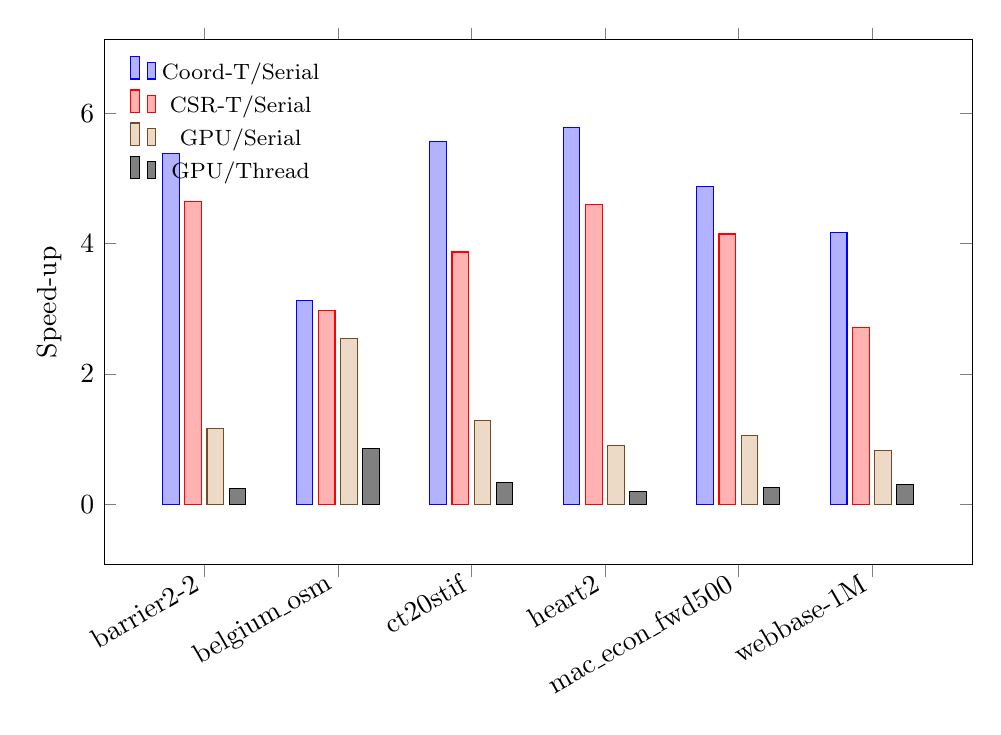
\begin{tikzpicture}
    \begin{axis}[
        ybar, bar width=6pt,
        ymin=0, ymax=6.2,
        width=\columnwidth/1.1,
        height=0.55\columnwidth,
        scale only axis=true,          % <-- NEW
        enlargelimits=0.15,
        symbolic x coords={1,2,3,4,5,6},
        xticklabels={
            barrier2-2,
            belgium\_osm,
            ct20stif,
            heart2,
            mac\_econ\_fwd500,
            webbase-1M},
        xtick=data,
        x tick label style={rotate=30,anchor=east},
        ylabel={Speed-up},
        legend style={
      at={(0.02,0.98)},          % inside; near top-left
      anchor=north west,
      draw=none,                 % no border
      fill=none,
      font=\footnotesize,},
      ]
      % --- data using the numeric x=1…6 trick ---
      \addplot coordinates {(1,5.384) (2,3.124) (3,5.564) (4,5.786) (5,4.884) (6,4.169)};
      \addplot coordinates {(1,4.649) (2,2.969) (3,3.872) (4,4.606) (5,4.149) (6,2.709)};
      \addplot coordinates {(1,1.158) (2,2.551) (3,1.281) (4,0.902) (5,1.057) (6,0.825)};
      \addplot coordinates {(1,0.249) (2,0.859) (3,0.331) (4,0.196) (5,0.255) (6,0.304)};
      \legend{Coord-T/Serial, CSR-T/Serial, GPU/Serial, GPU/Thread}
    \end{axis}
  \end{tikzpicture}
  \caption{Relative performance of SpMV variants per matrix (higher is better).}
  \label{fig:spmv_speedup_bars}
\end{figure}



  \subsection{Related Work}

 Related to programming for the Raspberry Pis GPU, there is has been little work done. 
 The book "Raspberry Pi GPU Audio Video Programming" by Jan Newmarch looks at writing 
 programs for the GPU through OpenGL, OpenMAX, and OpenVG\cite{newmarch2017raspberry}. It looks at GPU programming 
 through the audio and video points of view rather than programming to the GPU as 
 a general purpose device. There are also a myriad of Papers that look Fast Fourier Transformations 
 (FFTs) utilizing the GPU. These studies utilize GPU\_FFT, a program written by Andrew Holme in 2014\cite{holme_gpu_fft}.
 This implementation was written directly in bytecode to utilize the V3D block of the BCM2835, the chip 
 of the Raspberry Pi 1. A spinoff paper also looked at a Vulkan FFT implementation to leverage the GPU\cite{he_comparing_2018}. 
 There have been papers which look at Optimizing OpenCL code for the Raspberry Pi. However, these papers
 look at writing OpenCL code that efficiently maps to the Pi's CPU.

 One paper which takes our proposed approach of compiling OpenCL code to Vulkan compute shaders using clvk\cite{vasileiou_accelerated_nodate}.
 Their research was on using heterogeneous systems to reconstruct 3D microwave tomography images from measuring 
 electromagnetic signals. Their paper states their research can benefit from relatively low power portable technology. 
 When running on the Raspberry Pi 4, their algorithm took over twice as long to run on the VideoCore VI as it took 
 to run on the Raspberry Pi's CPU. 

 This area of research heavily reflects research done in the mid 2000's to bring general purpose compute to 
 graphics hardware. During that time, GPUs where advancing from 8 bit chanel color value pipelines to 
 fully programmable vectorized floating point operation pipelines\cite{owens_survey_2007}. GPUs of this time 
 structure their computation into heavily parallelized graphics pipelines consisting of vertex operations, 
 privative assembly, rasterization, fragment operations, and compression into an image. The common languages to 
 interface with the GPU at the time where all based on the idea that the GPU would generate images. Such examples 
 of languages included Cg, HLSL, OpenGL, and Sh. At this time there where early languages and libraries which attempted 
 to map mathematical operations on memory (kernels) to shader streams.  Such examples included Accelerator by Microsoft 
 Research, CGiS, and Brook Programming Language. Early papers from this time explored crucial data parallel 
 tasks and data structures such as map, reduce, scatter and gather, sorting, dense arrays, sparse arrays, 
 and dynamic sparse arrays. Combining these ideas, complex algorithms are explored on GPUs such as differential 
 equations, linear algebra, and data queries. 
 
 As seen in the case of the microwave tomography images study, simply having access to heavily parallel hardware 
 does not guarantee an improvement in performance. Since the hardware of the Raspberry Pi is specifically tailored 
 to rendering graphics similar to early GPUs, we hypothesize that modern optimizations may not all work. 
 Looking further into specific optimizations made during the era of early general purpose GPU programming will likely
 be the best source help when programming for the Pi. 


 \section{Conclusion}

 In summary, this proposal aims to explore the untapped potential of the Raspberry Pi 5’s embedded GPU for 
 accelerating neural network inference. By leveraging the Broadcom VideoCore VII through a strategic porting 
 of OpenCL kernels to Vulkan, the research intends to address key challenges related to latency and power 
 consumption in edge computing environments. While preliminary expectations suggest that the performance 
 improvements may be incremental due to inherent architectural constraints, the insights gained will provide a 
 foundation for future optimizations and potential adaptations to other embedded platforms. Ultimately, this 
 work seeks to contribute to the broader field of Industry 4.0 by enhancing the computational capabilities of 
 low-cost, low-power devices, thus opening new avenues for real-time, on-device intelligence.
 
 \bibliographystyle{IEEEtran}  % or another style, e.g., plain, unsrt, etc.
 \bibliography{5234ProjectProposal}
 
 
 \vspace{12pt}
 
 \end{document}
 